\section{Метод золотого сечения}

\textbf{Метод золотого сечения} — это эффективный и простой способ нахождения локального минимума функции на заданном отрезке, за счет того, что на очередной итерации требует вычисления значения функции только в одной точке, что можеть быть очень важно, для сложновычислимых функций.

\begin{remark*}
Метод золотого сечения находит глобальный минимум только в случае унимодальных функций.
\end{remark*}

\begin{definition*}
Функция \textbf{унимодальная} на отрезке $[a, b]$, если $\exists \alpha, \beta: a\leq \alpha \leq \beta \leq b$ такие, что:

\begin{itemize}
    \item на отрезке $[a, \alpha]$ функция монотонно убывает
    \item на отрезке $[\beta, b]$ функция монотонно возрастает
    \item $\forall x \in [\alpha, \beta]: f(x) = \min\limits_{x\in[a,b]}f(x)$
\end{itemize}

\begin{figure}[h]
\centering
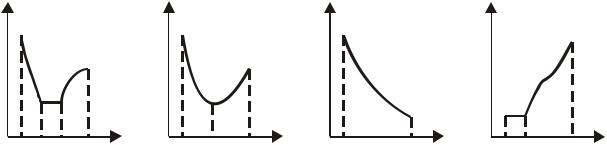
\includegraphics[scale=0.5]{unimodal_functions.jpg}
\caption{Примеры унимодальных функций}
\end{figure}
\end{definition*}

\textbf{Свойство.} Любой локальный минимум будет являться одновременно и глобальным минимумом.\\

\begin{wrapfigure}{l}{0.25\textwidth}
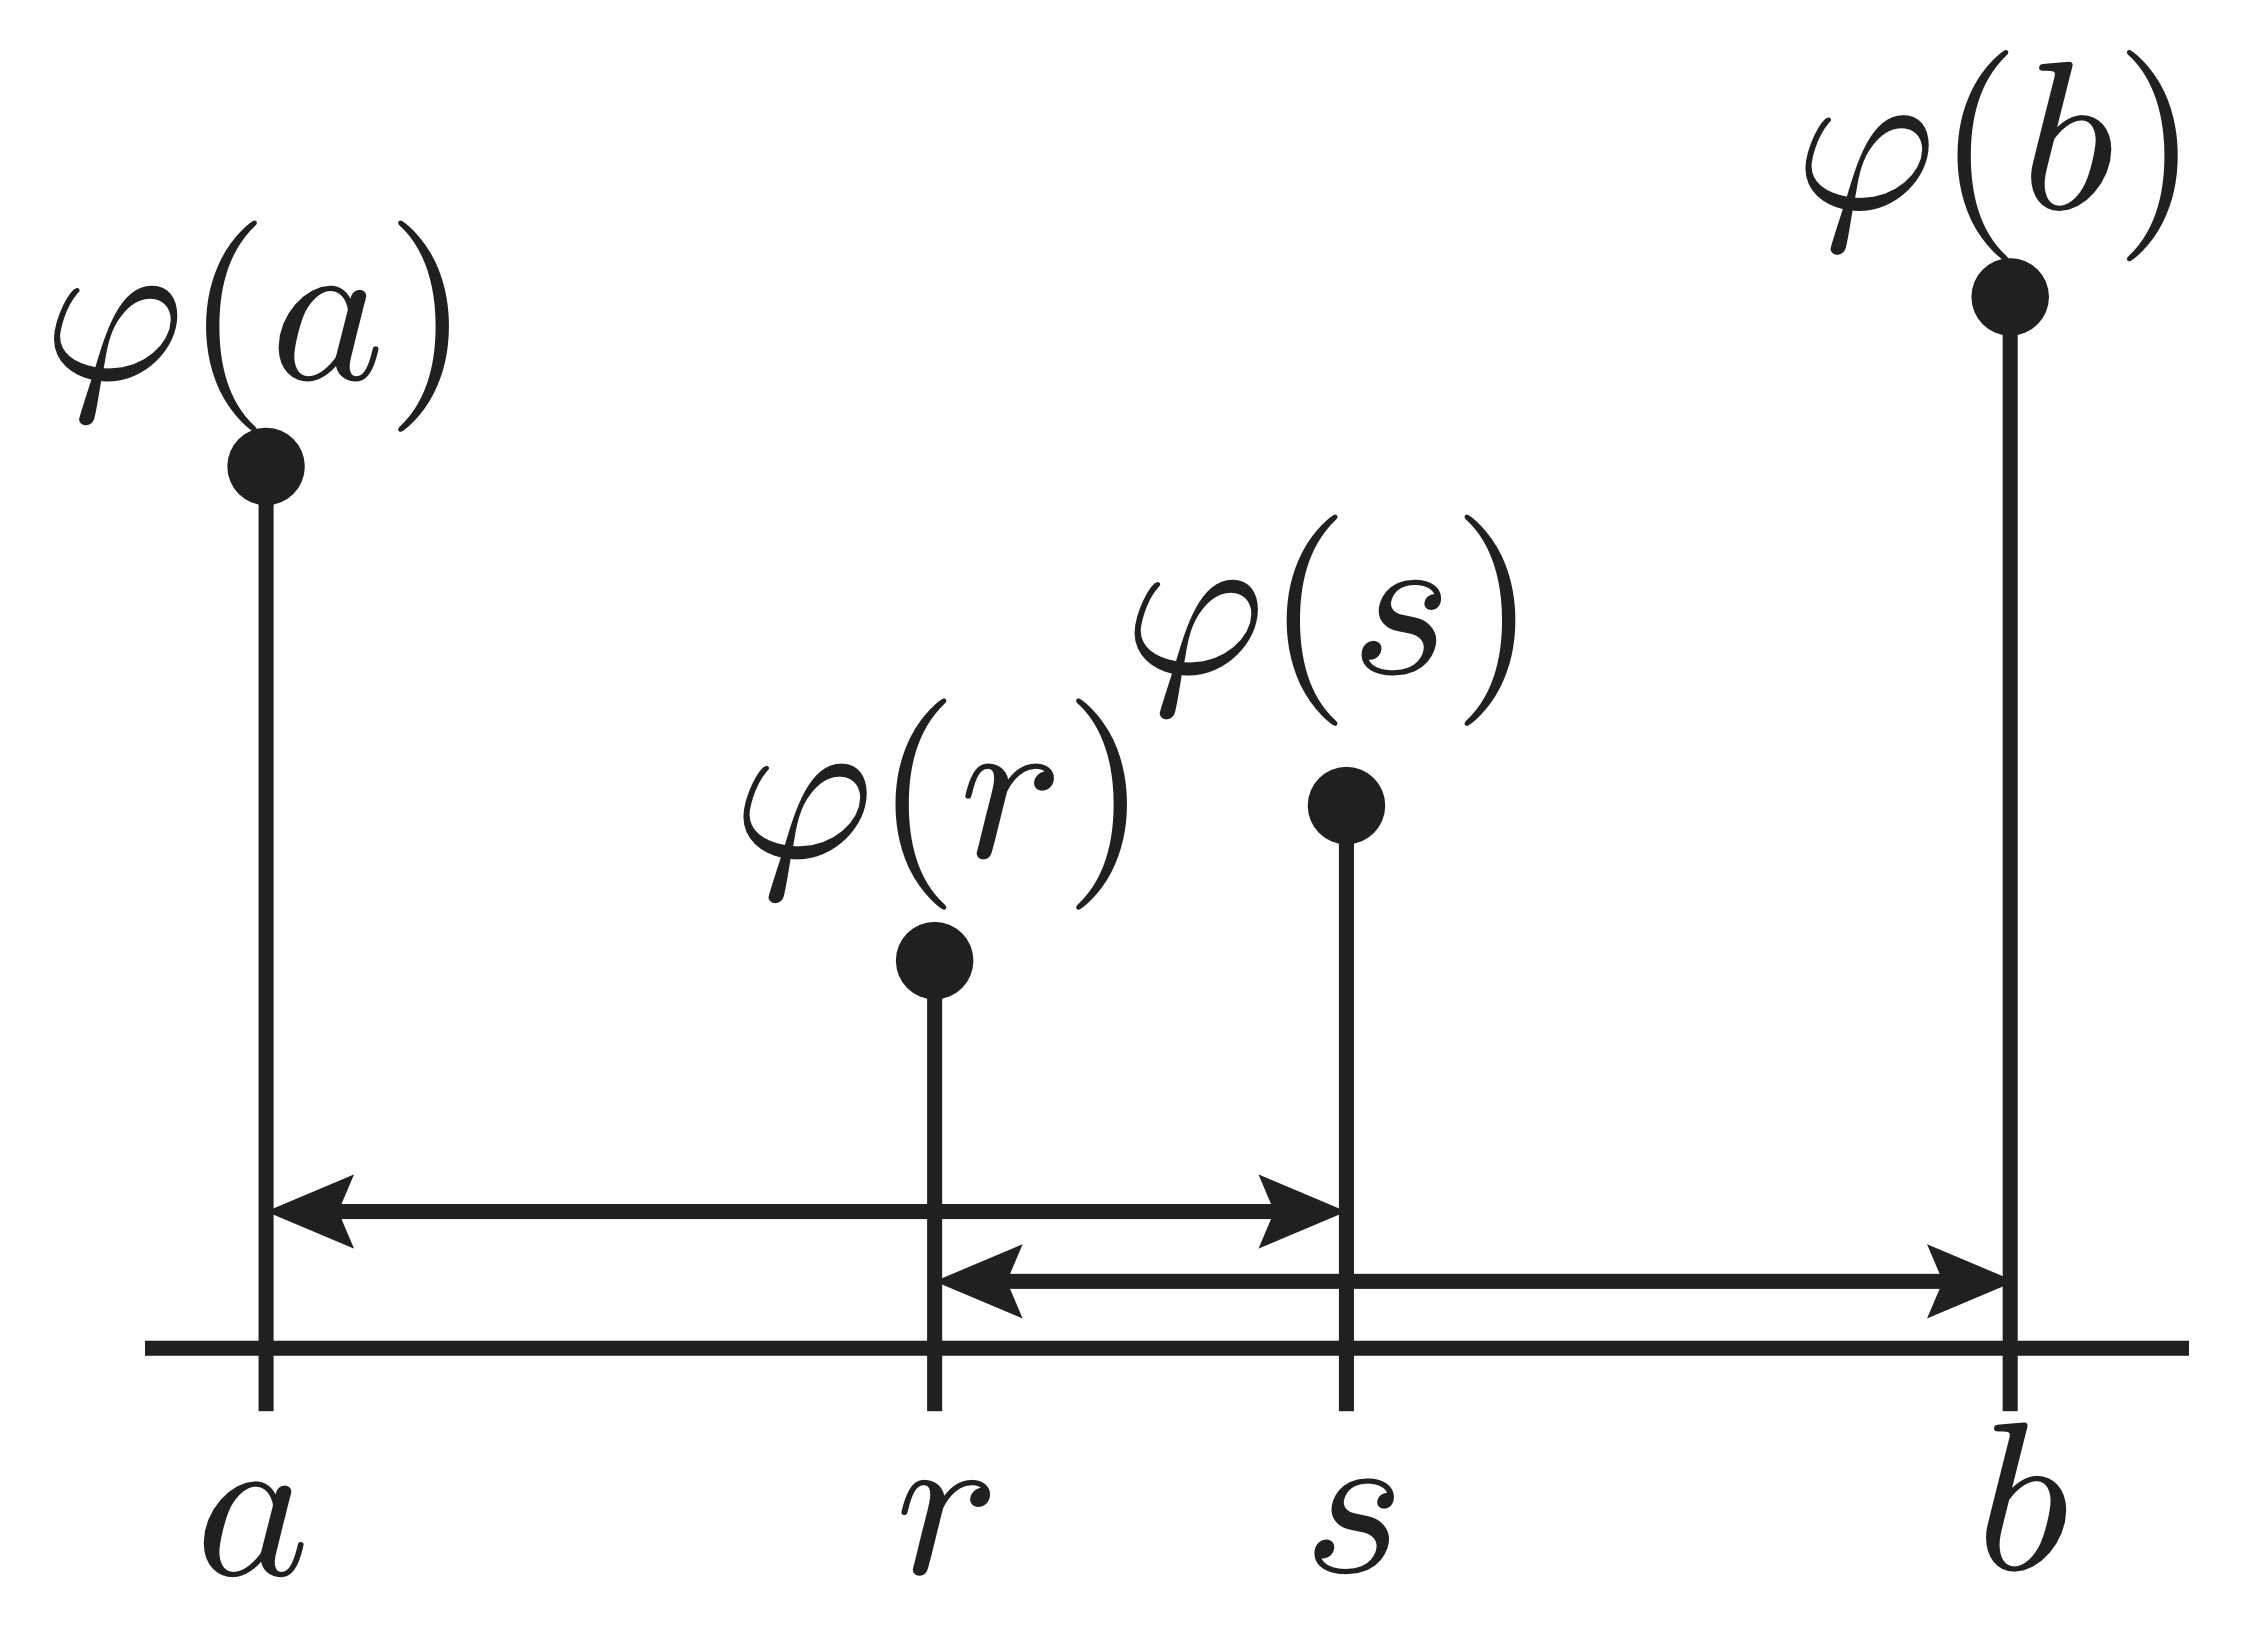
\includegraphics[width=0.9\linewidth]{golden_section.png} 
\caption{Итерация}
\label{fig:wrapfig}
\end{wrapfigure}

\textbf{Алгоритм.} Пусть хотим найти минимум функции $\varphi$ на отрезке $[a, b]$, разобъем его на три части двумя точками $r, s$ так, чтобы при отсекании одного из крайних подотрезков, одна из точек стала границей подотрезка для следующей итерации, то есть соотношение длин подотрезков оставалось прежним:\\

$|[a, r]|=|[s, b]|=l_1$

$|[r, s]|=l_2$

тогда, если $\varphi(r) \leq \varphi(s)$, то $s$ станет правой границей рассматриваемого отрезка, а $r$ станет правой внутренней точкой:\\

$$\frac{|[a, s]|}{|[a, b]|} = \frac{|[a, r]|}{|[a, s]|} \Rightarrow \frac{l_1+l_2}{2l_1+l_2} = \frac{l_1}{l_1+l_2} \Rightarrow l_1^2-l_1\cdot{l_2}-l_2^2=0 \Rightarrow \frac{l_1}{l_2}=\frac{1+\sqrt{5}}{2}=\Phi \approx 1.618$$\\

\begin{remark*}
Число $\Phi$ называют \textbf{золотым сечением}
\end{remark*}

Несмотря на то, что данный метод гарантированно находит глобальный минимум только для унимодальных функций, мы будем его использовать для сравнения с более надежными методами.

\textbf{Реализация}\\

\begin{lstlisting}[language=Python]
def GoldenRatio(func_index, index, a, b, p, e_d, e_f):  # f(function), i(index of direction),
    # a(left border), b(right border), p(current point), e_d(error of d), e_f(error of f)
    F = Functions[func_index * 2]
    phi = (1 + np.sqrt(5)) / 2  # constant of golden ratio
    x_1 = b - (b - a) / phi
    x_2 = a + (b - a) / phi
    p_1 = p.copy()  # current point
    p_2 = p.copy()  # current point
    p_1[index] = x_1
    p_2[index] = x_2
    f_1 = F(p_1)  # value in 1-st point
    f_2 = F(p_2)  # value in 2-nd point
    while (b - a > e_d) | (abs(f_1 - f_2) > e_f):  # termination criteria
        if f_1 <= f_2:
            b = x_2
            x_2 = x_1
            x_1 = b - (b - a) / phi

            p_1[index] = x_1
            p_2[index] = x_2

            f_2 = f_1
            f_1 = F(p_1)
        else:
            a = x_1
            x_1 = x_2
            x_2 = a + (b - a) / phi

            p_1[index] = x_1
            p_2[index] = x_2

            f_1 = f_2
            f_2 = F(p_2)

    best_point = []
    for i in range(len(p)):
        best_point.append((p_1[i] + p_2[i]) / 2)

    return best_point  # point of extremum with error e_d
\end{lstlisting}

\textbf{Сложность}\\

На каждой итерации длина рассматриваемого отрезка умножается на $$\frac{l_1+l_2}{l_1+l_2+l_2}=\frac{3+\sqrt{5}}{4+2\sqrt{5}}=\Phi^{-1} = \phi$$\\
Для достижения точности $\delta$ потребуется $$\frac{\ln(\frac{|[a, b]|}{\delta})}{\ln(\Phi)} \approx 2\ln(\frac{|[a, b]|}{\delta})$$ итераций.